\documentclass[british,10pt]{beamer}
\usepackage{pifont}
\usepackage{listings}

% Beamer specific settings

% Other styles can be used instead of Boadilla, e.g., to add an index column.
\mode<presentation>
{
  \usetheme{Boadilla} % Without index, with footer
}

\title{Building a better VHDL testing environment}
\author[J. Guillaume]{Joren Guillaume}
\date[JAN'15, Gent]{Thesis presentation}
\institute[Ghent University]
{
  FEA\\
  Ghent University
}

% This command makes the logo appear at the right side which does not fit
% the UGent style. A solution is found further below.
% \logo{\includegraphics[scale=0.25]{logolabel.jpg}}

\AtBeginSection[]
{
  \begin{frame}<beamer>\frametitle{Outline}
    \tableofcontents[currentsection,currentsubsection]
  \end{frame}
}

\setbeamersize{text margin left=1cm}
\setbeamersize{text margin right=1cm}

\begin{document}


% Titlepage containing the logo of the Faculty (Engineering in this example)
\begin{frame}[plain]
\mode<presentation>{
\includegraphics[width=\textwidth]{tw.pdf}}
  \titlepage
\end{frame}


% UGent logo at left side from second slide on.
\setbeamertemplate{sidebar left}{ 
\vfill 
\rlap{%\hskip0.1cm 
 
\includegraphics[scale=0.3]{logolabel2.jpg} } 
\vskip10pt 
}

\begin{frame}<beamer>\frametitle{Outline}
  \tableofcontents
\end{frame}

\section{Situating}
\subsection{Testing VHDL}

%\begin{frame}\frametitle{VHDL}
%\begin{itemize}
%\item VHSIC Hardware Description Language
%\item Used for describing digital and mixed-signal systems 
%\item Developed by U.S. Department of Defense
%\begin{itemize}
%\item Document \ding{222} Simulate \ding{222} Synthesize
%\end{itemize}
%\end{itemize}
%\end{frame}
%
%\begin{frame}\frametitle{Testing VHDL}
%\begin{columns}
%\begin{column}{0.05\textwidth}
%\end{column}
%\begin{column}{0.55\textwidth}
%Test benches
%\begin{itemize}
%\item Unit Under Test (UUT)
%\item Signal coupling \& stimuli
%\item Output tracking
%\begin{itemize}
%\item Assertions
%\item Comparison to desired result
%\\(Manual or automated)
%\item Wave-check
%\end{itemize}
%\end{itemize}
%%\vspace{0.25cm}
%%Problems
%%\begin{itemize}
%%\item Non-standardized process
%%\item Single point of failure
%%\item Time consuming
%%\end{itemize}
%\end{column}
%\column{0.4\textwidth}
%\raggedleft
%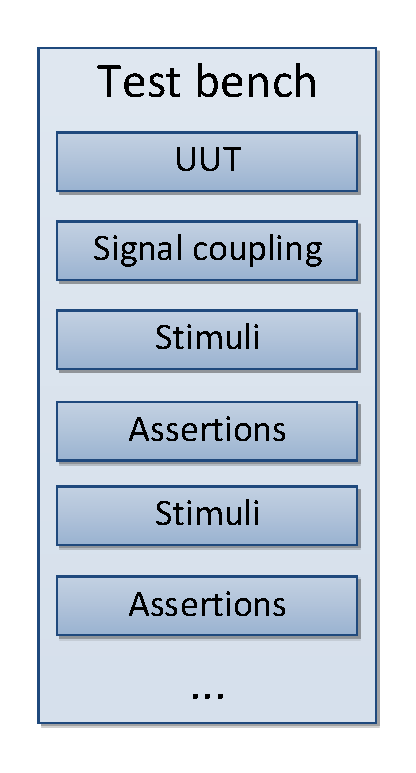
\includegraphics[width=\textwidth]{images/TB.pdf}
%\end{columns}
%\end{frame}

\begin{frame}\frametitle{Testing VHDL}
VHDL
\begin{itemize}
\item VHSIC Hardware Description Language
\item Develop hardware
\item Tested with test benches
\begin{itemize}
\item Output tracking
\end{itemize}
\end{itemize}
\vskip5pt
Problems
\begin{itemize}
\item Non-standardized process
\item Single point of failure
\item Time consuming
\end{itemize}
\end{frame}

\subsection{Software development techniques}
\begin{frame}\frametitle{Software development techniques}
\begin{columns}
\begin{column}{0.6\textwidth}
Unit testing
\begin{itemize}
\item Unit = smallest behaviour in code
\item Test failure \ding{222} exact location
\end{itemize}
\vskip3pt
Test First Development
\begin{itemize}
\item Create test before the code
\item How the code will behave?
\end{itemize}
\vskip3pt
Test Driven Development
\begin{itemize}
\item TFD \& short development cycle
\item Proven to significantly reduce errors
\end{itemize}
\end{column}
\column{0.4\textwidth}
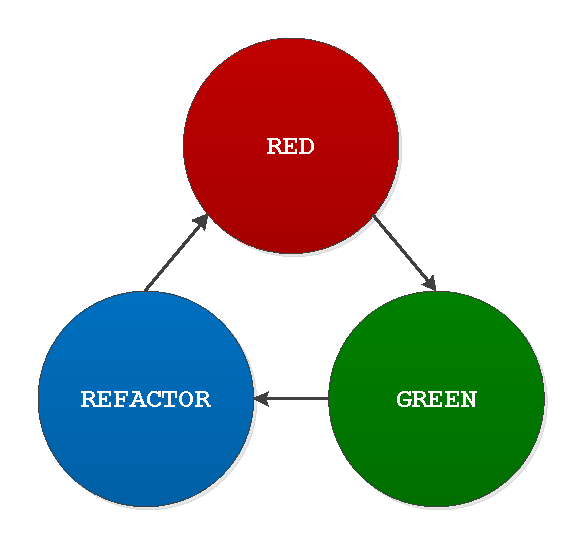
\includegraphics[width=\textwidth]{images/tdd.pdf}
\end{columns}
\end{frame}

%\subsection{Proposed solution}
%
%\begin{frame}\frametitle{Proposed solution}
%Standardized testing framework
%\begin{itemize}
%\item Based on software development techniques
%\item Cross platform
%\item Utility library
%\item Continuous Integration system
%\item At the core: Python script
%\end{itemize}
%\end{frame}

%\begin{frame}\frametitle{VHDL - design flow}
%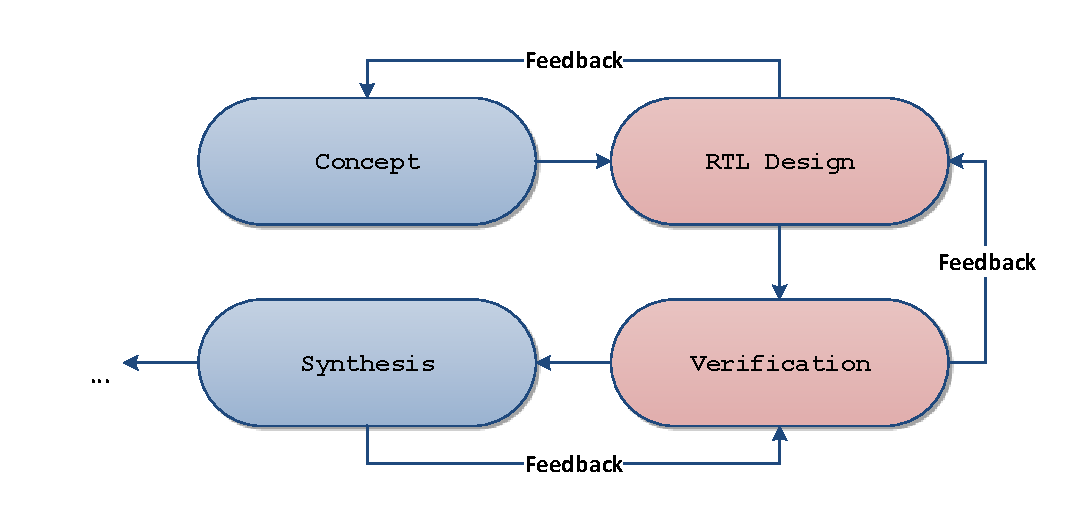
\includegraphics[width=\textwidth]{images/designflow2.pdf}
%\end{frame}

%\begin{frame}[fragile]\frametitle{Testing VHDL - assertions example }
%D-flipflop
%\begin{itemize}
%\item d: delay, input
%\item q: output
%\end{itemize}
%\centering
%\begin{lstlisting}[language=VHDL, tabsize=4, frame=single, framesep=2mm, belowskip=8pt, aboveskip=8pt, showstringspaces=false, basicstyle=\scriptsize]
%	...
%		assert q = '0'
%			report "Wrong output value at startup" severity FAILURE;
%		d <= '1';
%     	WAIT FOR clk_period;
%     	assert q = '1'
%			report "Wrong output value at first test" severity FAILURE;
%	...
%\end{lstlisting}
%\end{frame}

%\subsection{Software development techniques}

%\begin{frame}\frametitle{Unit testing}
%Unit testing
%\begin{itemize}
%\item Unit: smallest behaviour in code
%\item Unit test: Tests that behaviour
%\item Test success/failure \ding{222} excellent locator
%\end{itemize}
%\end{frame}

%\begin{frame}\frametitle{Unit testing}
%Unit testing
%\begin{itemize}
%\item Unit: smallest behaviour in code
%\item Unit test: Tests that behaviour
%\item Test success/failure \ding{222} excellent locator
%\end{itemize}
%\end{frame}
%
%\begin{frame}\frametitle{Test Driven Development}
%\begin{columns}
%\begin{column}{0.6\textwidth}
%Test Driven Development
%\begin{itemize}
%\item Software development technique
%\item Proven to significantly reduce errors
%\item All behaviour is tested
%\item Unit testing \& short development cycle
%\item Red - Green - Refactor
%\end{itemize}
%\end{column}
%\column{0.4\textwidth}
%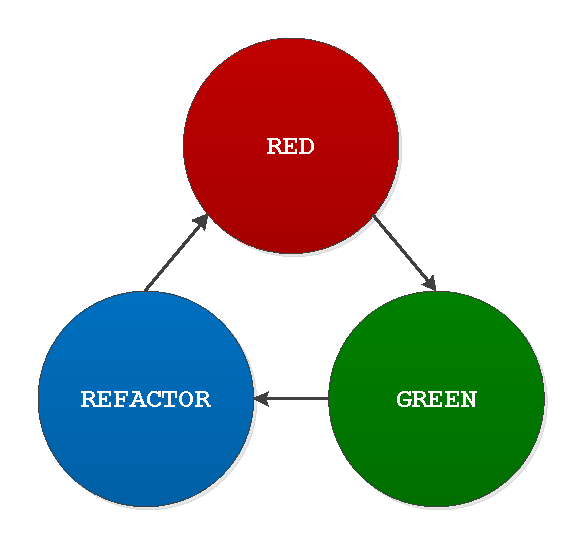
\includegraphics[width=\textwidth]{images/tdd.pdf}
%\end{columns}
%\end{frame}

%\begin{frame}\frametitle{TDD - design flow}
%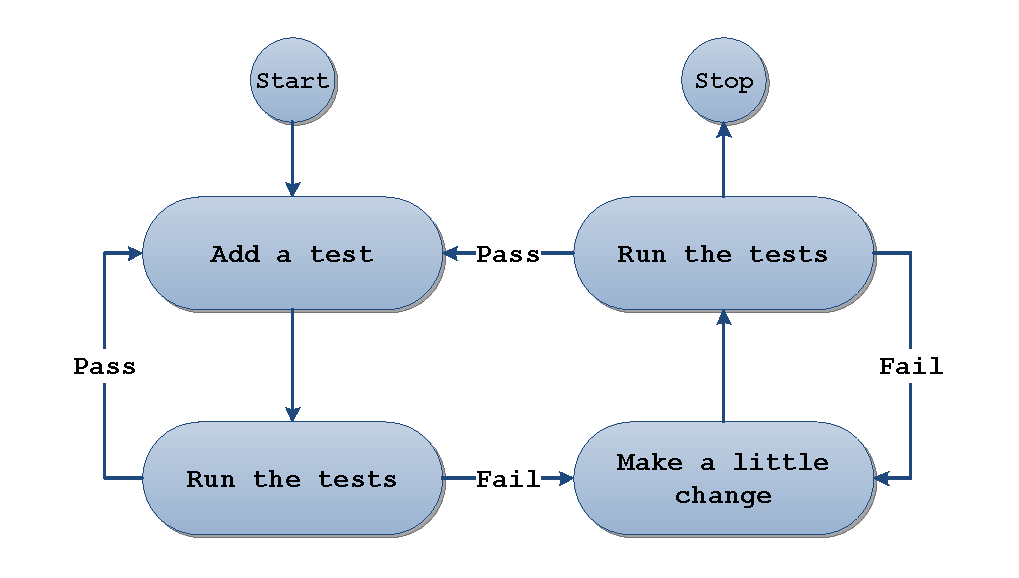
\includegraphics[width=\textwidth]{images/TDDflow2.pdf}
%\end{frame}

\section{Proposed solution}
\subsection{VHDL testing framework}

\begin{frame}\frametitle{VHDL testing framework}
Python script
\begin{enumerate}
\item Identify and group tests
\item Separate groups into new test benches
\item Compile sources
\item Compile and execute new test benches
\item Capture and process results
\end{enumerate}
\end{frame}

\subsection{Preparing test benches}
\begin{frame}\frametitle{Preparing test benches}
\begin{columns}
\begin{column}{0.6\textwidth}
\begin{itemize}
\item Use Bitvis utility library
\begin{itemize}
\item Faster coding
\item Improved readability
\end{itemize}
\item Separate independent tests
\begin{itemize}
\item Line by line
\item Start/Stop
\item Partitioned
\end{itemize}
\item Create commands file
\end{itemize}
%\hskip24pt\ding{222} Unit testing
\end{column}
\column{0.4\textwidth}

\includegraphics[width=0.8\textwidth]{images/bitvis.png}
\end{columns}
\end{frame}

\begin{frame}[fragile]\frametitle{Modified test bench example}
D flip-flop
\begin{itemize}
\item Old test bench:
\end{itemize}
\begin{lstlisting}[language=VHDL, tabsize=4, frame=single, framesep=2mm, belowskip=5pt, aboveskip=5pt, showstringspaces=false, basicstyle=\scriptsize]
assert q = '0'
    report "Wrong output value at startup" severity FAILURE;
d <= '1';
WAIT FOR clk_period;
assert q = '1'
    report "Wrong output value at first test" severity FAILURE;
\end{lstlisting}
\vskip1pt
\begin{itemize}
\item Modified test bench:
\end{itemize}
\begin{lstlisting}[language=VHDL, tabsize=4, frame=single, framesep=2mm, belowskip=5pt, aboveskip=5pt, showstringspaces=false, basicstyle=\scriptsize]
--Test 1
    check_value(q = '0', FAILURE, "Wrong output value at startup");
    write(d, '1', "DFF");
    check_value(q = '1', FAILURE, "Wrong output value at first test");
    ...
--End 1
\end{lstlisting}
\end{frame}

\subsection{Processing and compilation}
\begin{frame}\frametitle{Processing and compilation}
Python script:
\begin{enumerate}
\item Read command line arguments
\item Read modified test bench
\item Group tests into new test benches
\end{enumerate}
ModelSim:
\begin{enumerate}
\setcounter{enumi}{3}
\item Compile source code
\item Compile test benches
\end{enumerate}
\end{frame}

\subsection{Execution and results}
\begin{frame}\frametitle{Execution and results}
ModelSim:
\begin{enumerate}
\item Execute separated test benches
\end{enumerate}
Python script:
\begin{enumerate}
\setcounter{enumi}{1}
\item Capture ModelSim output
\item Process results
\begin{itemize}
\item Text report
\item XML report
\end{itemize}
\end{enumerate}
\end{frame}

\begin{frame}\frametitle{Automation}
\begin{columns}
\begin{column}{0.6\textwidth}
Hudson-CI
\begin{itemize}
\item Source at revision control system
\item Create job per project
\item Get latest version from RC
\item Timed script execution
\item Result progress (XML)
\end{itemize}
\end{column}
\column{0.4\textwidth}

\includegraphics[width=0.8\textwidth]{images/hudson.png}
\end{columns}
\end{frame}

%\subsection{Utility library}
%
%\begin{frame}\frametitle{Utility library}
%\begin{columns}
%\begin{column}{0.6\textwidth}
%Bitvis utility library
%\begin{itemize}
%\item Compatible with all VHDL versions
%\item Expands VHDL functions
%\begin{itemize}
%\item Easy value checking
%\item Formatted output
%\end{itemize}
%\item Quick \& uniform coding
%\begin{itemize}
%\item Reduces time spent coding
%\item Improves readability
%\end{itemize}
%\end{itemize}
%\end{column}
%\column{0.4\textwidth}
%
\includegraphics[width=0.8\textwidth]{images/bitvis.png}
%\end{columns}
%\end{frame}

%\subsection{Continuous Integration}
%
%\begin{frame}\frametitle{Continuous Integration}
%\begin{columns}
%\begin{column}{0.6\textwidth}
%Hudson-CI
%\begin{itemize}
%\item Centralized, automated testing
%\begin{itemize}
%\item Revision control
%\item Timed building
%\end{itemize}
%\item Easy to read results
%\item Very customizable
%%\item Standardized test reports (XML)
%%\item Displays statistics
%\end{itemize}
%\end{column}
%\column{0.4\textwidth}
%
\includegraphics[width=0.8\textwidth]{images/hudson.png}
%\end{columns}
%\end{frame}

%\subsection{Python script}
%
%\begin{frame}\frametitle{Python script}
%Test bench parser
%\begin{itemize}
%\item Separates independent tests
%\begin{itemize}
%\item Remove single point of failure
%\end{itemize}
%\item Customizable
%\begin{itemize}
%\item Command-line arguments
%\end{itemize}
%\item Multiple useful outputs
%\begin{itemize}
%\item Processed text-based report
%\item Processed XML report
%\end{itemize}
%\end{itemize}
%\end{frame}
%
%\begin{frame}\frametitle{Script workflow}
%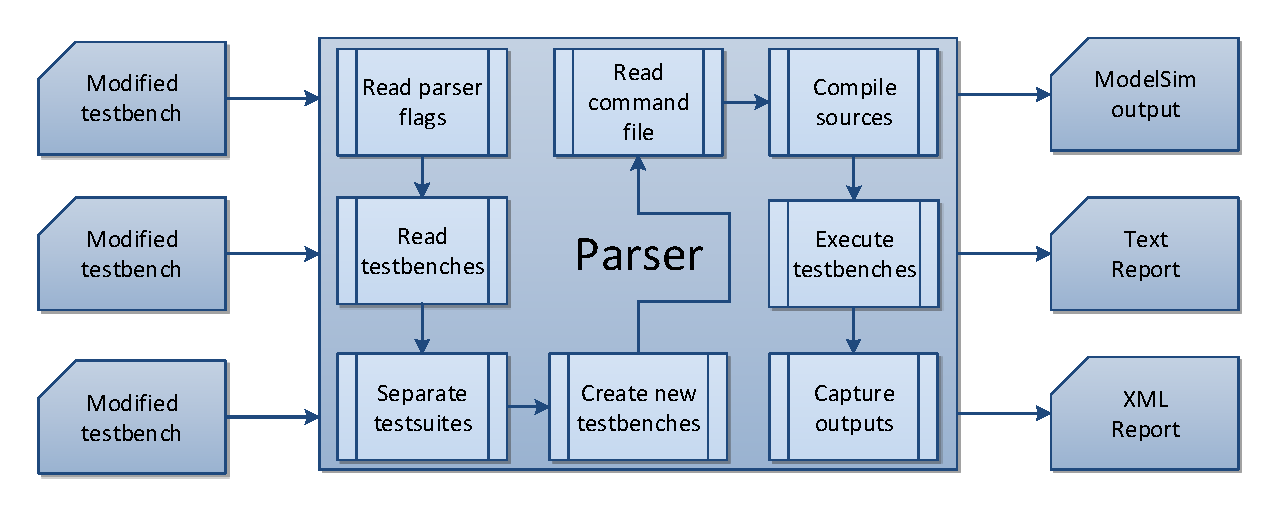
\includegraphics[width=\textwidth]{images/parserwork.pdf}
%\newline{}
%\centering(Steps of the parser logged separately)
%\end{frame}


%\subsection{Using the framework}
%
%\begin{frame}\frametitle{Using the framework}
%Preparing the test bench
%\begin{enumerate}
%\item Import the utility library
%\item Decide on separation method
%\begin{itemize}
%\item Line by line \ding{222} No editing test bench
%\item Start/Stop
%\item Partitioned (recommended)
%\end{itemize}
%\item Create command file
%\end{enumerate}
%\end{frame}


%\begin{frame}[fragile]\frametitle{Modified test bench example}
%D flip-flop
%\begin{itemize}
%\item Old test bench:
%\end{itemize}
%\begin{lstlisting}[language=VHDL, tabsize=4, frame=single, framesep=2mm, belowskip=5pt, aboveskip=5pt, showstringspaces=false, basicstyle=\scriptsize]
%assert q = '0'
%    report "Wrong output value at startup" severity FAILURE;
%d <= '1';
%WAIT FOR clk_period;
%assert q = '1'
%    report "Wrong output value at first test" severity FAILURE;
%\end{lstlisting}
%\vskip1pt
%\begin{itemize}
%\item Modified test bench:
%\end{itemize}
%\begin{lstlisting}[language=VHDL, tabsize=4, frame=single, framesep=2mm, belowskip=5pt, aboveskip=5pt, showstringspaces=false, basicstyle=\scriptsize]
%--Test 1
%    check_value(q = '0', FAILURE, "Wrong output value at startup");
%    write(d, '1', "DFF");
%    check_value(q = '1', FAILURE, "Wrong output value at first test");
%    ...
%--End 1
%\end{lstlisting}
%\end{frame}


%\begin{frame}[fragile]\frametitle{Using the framework}
%Running Hudson-CI
%\begin{enumerate}
%\item Create new job
%\item Optional: set for import from revision control source
%\item Set correct parser flags in shell command
%\item Build \& check results
%\end{enumerate}
%\vskip5pt
%\begin{lstlisting}[language=bash, tabsize=4, frame=single, framesep=2mm, belowskip=8pt, aboveskip=8pt, showstringspaces=false, basicstyle=\scriptsize]
%python src\testbench_parser.py -m partitioned -l sim\tb_dff_r.vhd
%\end{lstlisting}
%\end{frame}

%\begin{frame}[fragile]\frametitle{Job example}
%\begin{lstlisting}[language=bash, tabsize=4, frame=single, framesep=2mm, belowskip=8pt, aboveskip=8pt, showstringspaces=false, basicstyle=\scriptsize]
%$ python src\testbench_parser.py -m partitioned -l sim\tb_dff_r.vhd
%\end{lstlisting}
%\end{frame}


%\begin{frame}\frametitle{Framework design flow}
%\centering
%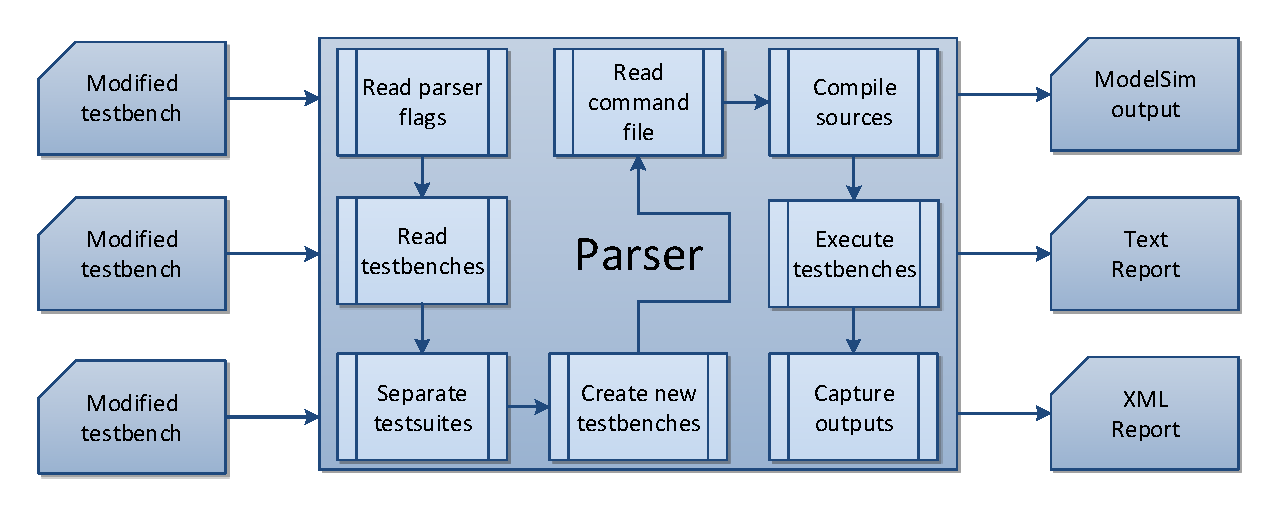
\includegraphics[width=\textwidth]{images/parserwork.pdf}
%\end{frame}

\section{Concluding}

\subsection{Results}
\begin{frame}\frametitle{Results}
\begin{itemize}
\item Multiple open-source projects converted
\end{itemize}
\medskip
{\centering
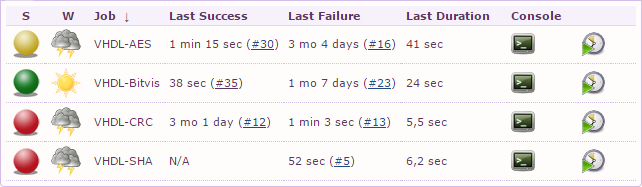
\includegraphics[width=\textwidth]{images/jobs.png}}
%\\\hskip10pt\ding{222} Bypassed single point of failure
%\\\hskip10pt\ding{222} Automated testing = faster development
%\\\hskip10pt\ding{222} Successful runs when VHDL code OK
%\\\hskip10pt\ding{222} Partially completed test-runs even with faults in code
%\\\hskip10pt\ding{222} Unsuccessful runs only due to compilation errors\\
\end{frame}


%\begin{frame}\frametitle{Results}
%{\centering
%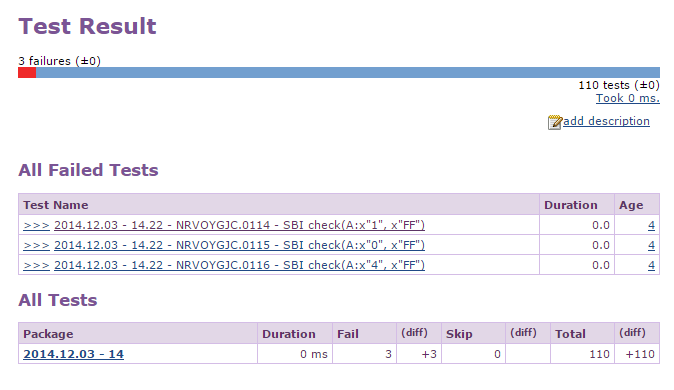
\includegraphics[width=.85\textwidth]{images/results1.png}}
%\end{frame}
%
%\begin{frame}\frametitle{Results}
%{\centering
%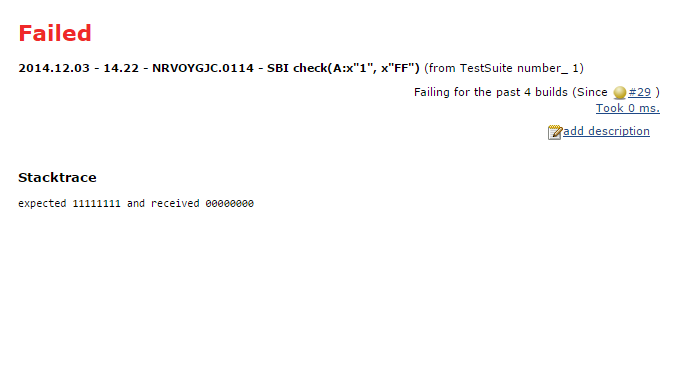
\includegraphics[width=.85\textwidth]{images/results2.png}}
%\end{frame}
%%\item Code duplication increases compile \& simulation time

\subsection{Future work}

\begin{frame}\frametitle{Future work}
\begin{itemize}
\item Wider, better tool support
\item Lexical analysis
\begin{itemize}
\item Automated partitioning
\item Smart test bench generation
\end{itemize}
\item Adapted CI tool
\begin{itemize}
\item Specific needs of hardware development
\end{itemize}
\end{itemize}
\end{frame}
%%VOLGENDE
%%STAP
%%IN
%%DEZE
%%ONTWIKKELING
%%WAT
%%NU?


\begin{frame}\frametitle{Thanks for your attention}
\centering
\Huge Questions?
\end{frame}

%\begin{frame}\frametitle{Commentaries on developing VHDL}
%\begin{itemize}
%\item Outdated practices
%\begin{itemize}
%\item An industry stuck in 1993
%\item "Don't fix what isn't broken"
%\end{itemize}
%\item Hardware engineers are not software developers
%\begin{itemize}
%\item Little to no software development experience
%\item Taught by seniors at work
%\end{itemize}
%\item VHDL has no reflection or introspection
%\begin{itemize}
%\item Could make test benches even more compact
%\end{itemize}
%\end{itemize}
%\end{frame}
%
%\subsection{Conclusion}
%
%\begin{frame}\frametitle{Conclusion}
%\begin{itemize}
%\item Software methods are applicable to an extent if:
%\begin{itemize}
%\item Tailored to development needs
%\item Integrated with existing methods
%\end{itemize}
%\item Framework provided:
%\begin{itemize}
%\item Easier to read code
%\item Precise debugging information
%\item Faster development
%\end{itemize}
%\end{itemize}
%\end{frame}

\section{Demo}
\begin{frame}\frametitle{Demo}
\centering
\Huge Demo
\end{frame}

\end{document}
